\chapter{Generazione degli APK}
\label{genapk}
\lhead{Generazione degli APK}
In questo capitolo verrà analizzato il processo di generazione dell'APK dell'applicazione (\emph{app.apk} nella relazione) e dell'APK di test (\emph{test.apk} nella relazione), entrambi file di input per la funzionalità di automazione dei test. In particolar modo, la generazione verrà affrontata nei seguenti passi:
\begin{itemize}[nosep]
\item Creazione della classe di test 
\item Parametrizzazione della classe di test
\item Generazione dei file APK
\end{itemize}
\noindent Al termine del capitolo verrà dedicata una sezione (Sezione \ref{genapknocod}) alla generazione dei file APK nel caso in cui non si disponga del codice sorgente.

\section{Creazione della classe di test}
\rhead{Creazione della classe di test}
\label{creazioneclassetest}
Il primo step da affrontare nella generazione degli APK riguarda la creazione della classe che contiene, come unico caso di test, il caso di test in grado di riprodurre il bug. Una volta aperto il progetto dell'applicazione in Android Studio (Appendice A - Android Studio), la classe può essere:
\begin{itemize}[nosep]
\item [$\blacksquare$]\textbf{scritta manualmente} \newline
Utilizzando la libreria Espresso (Appendice A - Espresso)
\item [$\blacksquare$]\textbf{registrata automaticamente} \newline
Utilizzando lo strumento, già integrato nell’editor, Espresso Test Recorder  (Appendice A - Espresso Test Recorder) (Appendice A - Registrazione del caso di test con Espresso Test Recorder) 
\end{itemize}
In ogni caso, la classe di test creata dovrà essere posizionata nella cartella "androidTest" (cartella generato automaticamente da Android Studio per contenere gli instrumented tests) visibile nella vista 'Android' di Android Studio (Figura \ref{fig:and.android.studio}).


\begin{figure}[H]
    \centering
    \begin{minipage}{0.4\textwidth}
        \centering
        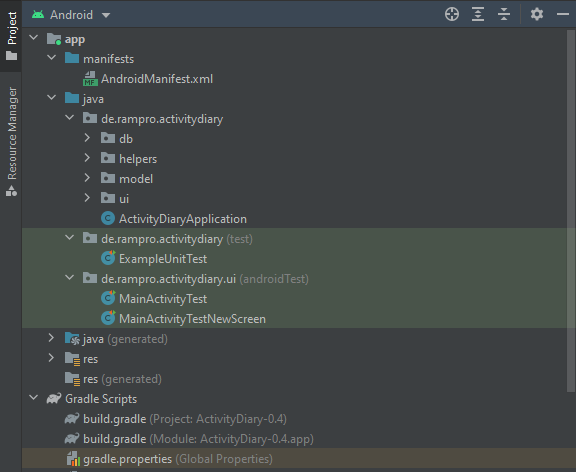
\includegraphics[scale=0.44]{and.android.studio} 
        \caption{Vista 'Android' in Android Studio - progetto 1}
            \label{fig:and.android.studio}
    \end{minipage}\hfill
    \begin{minipage}{0.5\textwidth}
        \centering
        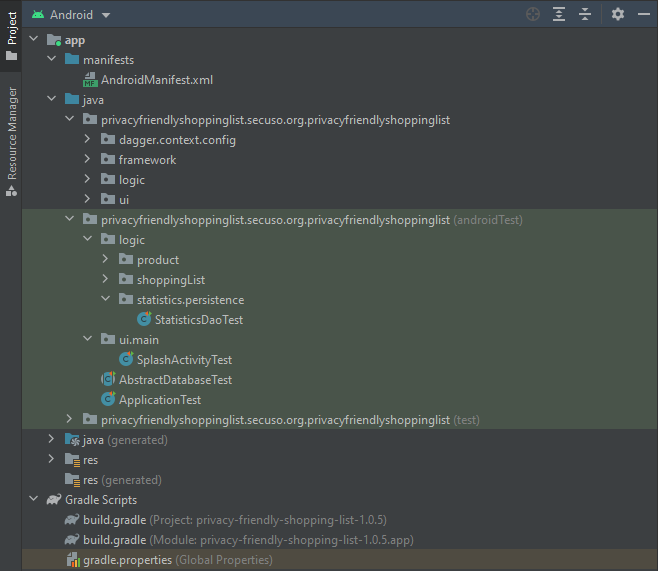
\includegraphics[scale=0.38]{and.2.android.studio} 
        \caption{Vista 'Android' in Android Studio - progetto 2}
            \label{fig:and.2.android.studio}
    \end{minipage}\hfill
\end{figure}

\bigskip
\noindent\textbf{Posizione della classe di test} \\
Il posizionamento della classe di test all'interno della cartella 'androidTest' influisce sul valore del parametro \emph{@class}, essenziale all'esecuzione della funzione di automazione dei test. In particolare:
\begin{itemize} [nosep]
\item [$\blacksquare$] \textbf{Caso 1} (consigliato) \newline
Nel caso in cui la classe sia posizionata nella radice (direttamente nella cartella 'androidTest'), il valore del parametro \emph{@class} dovrà semplicemente coincidere con il nome della classe di test.  \newline
\textcolor{gray}{Esempio - In Figura \ref{fig:and.android.studio}, nel caso in cui la classe contenente il caso di test che riproduce il bug sia 'MainActivityTest', il parametro \emph{@class} dovrà semplicemente assumere il valore 'MainActivityTest' }
\item [$\blacksquare$] \textbf{Caso 2} \newline
Nel caso in cui la classe sia posizionata in un package interno alla cartella 'androidTest', il valore del parametro \emph{@class} dovrà rispettare il pattern [pacchetto].[className] .  \newline
\textcolor{gray}{Esempio - In Figura \ref{fig:and.2.android.studio}, nel caso in cui la classe contenente il caso di test che riproduca il bug sia 'StatisticsDaoTest', il parametro \emph{@class} dovrà assumere il valore 'logic.statistics.persistence.StatisticsDaoTest' }
\end{itemize}

\section{Parametrizzazione della classe di test}
\label{paramclasstest}
\rhead{Parametrizzazione della classe di test}
Il secondo step da affrontare nella generazione degli APK riguarda la parametrizzazione della classe di test di cui la creazione è stata affrontata nella sezione precedente (Sezione \ref{creazioneclassetest}). Come analizzato nella Sezione \ref{pasparam}, nell'automazione dei test, per ogni lancio del test parametrico, i parametri vengono passati  alla strumentazione di test in formato JSON. Dalla classe di test si può avere accesso agli argomenti del bundle della strumentazione e quindi ai parametri di esecuzione.
\\\\
\noindent Per rendere la classe di test parametrica è necessario inserire, all'inizio di questa, il codice in Figura \ref{fig:parametrized};

\begin{figure}[H]
	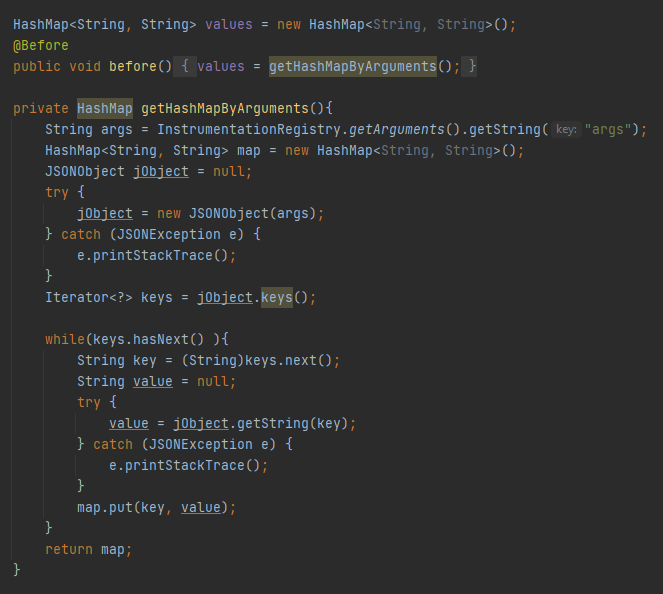
\includegraphics[scale=0.50]{parametrized}
	\centering
	\caption{Codice per la parametrizzazione delle classi di test}
    \label{fig:parametrized}
\end{figure}

\noindent Il funzionamento del codice, nel dettaglio, può essere sintetizzato come segue :
\begin{enumerate}[nosep]
\item dichiara e inizializza una hashmap (\emph{values});
\item prima di eseguire qualsiasi caso di test, assegna un nuovo valore alla struttura dati appena creata chiamando il metodo \emph{getHashMapByArguments()} che:
\begin{itemize} [nosep]
\item[1.] ottiene dalla strumentazione di test la stringa passata contenente i parametri in formato json;
\item[2.] dichiara e inizializza una nuova hasmap;
\item[3.] ricrea l'oggetto JSON dalla stringa ottenuta;
\item[4.] per ogni coppia chiave-valore dell'oggetto, aggiunge un elemento alla hasmap appena creata (con la stessa coppia chiave-valore);
\item[4.] ritorna l'hashmap;
\end{itemize}
\end{enumerate}
\bigskip
\noindent A questo punto, l'hasmpap \emph{values} contiene i parametri del test come coppia chiave-valore, in cui la chiave è rappresentata dall'etichetta della colonna del file di input a cui il valore fa riferimento. Si può quindi procedere alla parametrizzazione del caso di test in quanto l'hashmap \emph{values}  ha visibilità in tutta la classe.

\bigskip

\noindent Quindi, nei punti in cui il caso di test prevede l'inserimento di dati in input da parte dell'utente, il valore da inserire può essere ottenuto dall'hashmap specificando come chiave la colonna del file di input che contiene il dato  (\emph{values.get("inputColumnName")}). In Figura \ref{fig:esempio.parametrized} viene mostrato un esempio di parametrizzazione di un caso di test.

\begin{figure}[H]
	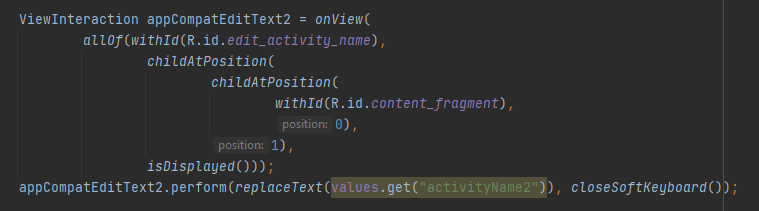
\includegraphics[scale=0.50]{esempio.parametrized}
	\centering
	\caption{Esempio: parametrizzazione della classe di test}
    \label{fig:esempio.parametrized}
\end{figure}

\section{Generazione dei file APK}
\rhead{Generazione dei file APK}
L'ultimo step riguarda la vera e propria generazione dei file \emph{app.apk} e \emph{test.apk}. Android Studio è in grado di generare i file richiesti automaticamente grazie all'integrazione di Gradle (Appendice A - Generazione degli APK) (Appendice A - Gradle). Al termine della generazione dei file, nell'Event Log di AS viene comunicata la directory in cui questi sono stati creati.  Solitamente il file che nella relazione è chiamato \emph{app.apk} viene generato come \emph{app-debug.apk}, mentre il file che nella relazione è chiamato \emph{test.apk} viene generato come \emph{app-debug-androidTest.apk}.


\section{Generazione degli APK senza disporre del codice sorgente}
\label{genapknocod}
\rhead{Generazione dei file APK senza disporre del codice sorgente}
Nelle sezioni precedenti è stata trattata la generazione degli APK supponendo di essere sempre in possesso del codice sorgente. In realtà, nella maggior parte dei casi, le applicazioni non sono open source e risulterebbe quindi utile poter utilizzare lo strumento anche nel caso in cui si disponga solamente dell'APK.  Il collega A. Mendieta, nella sua relazione di laurea triennale, ha trovato un metodo per la generazione dell'APK di test anche nel caso in cui non si possieda il codice sorgente (ma solo l'APK dell'applicazione), che ancora oggi è risultato utilizzabile.
\\\\
\noindent Brevemente, la soluzione individuata dal collega, utilizza un progetto open source (Appendice A - AndroidTestWithOutSource Project) che permette di generare solamente l'APK di test contenente la classe parametrizzata. In questo caso, la classe di test non può essere registrata con Espresso Test Recorder, ma deve essere scritta manualmente sfruttando le funzionalità offerte dallo strumento Ui Automator Viever (Appendice A - UI Automator Viewer). 
\\\\
\noindent Prima di poter utilizzare l'APK dell'applicazione e l'APK di test generata come file di input per il tool, risulta essenziale firmare gli APK con la stessa firma, operazioni facilmente effettuabile grazie allo strumento apksigner (Appendice A - apksigner).

